\documentclass[12pt,a4paper]{exam}

\usepackage[utf8]{inputenc}
\usepackage[T1]{fontenc}
\usepackage{amsmath}
\usepackage{amsfonts}
%\usepackage{amssymb}
\usepackage{graphicx}
\usepackage{geometry}
\usepackage{cancel}
\usepackage{enumitem}

\geometry{a4paper, margin=2cm}

\newcommand{\ito}{It$\hat{o}$}
\newcommand{\expect}[1]{\mathbb{E}^\mathbb{#1}}
\newcommand{\expectt}[2]{\mathbb{E}_{#2}^\mathbb{#1}}

\usepackage{cprotect}

\usepackage{xcolor}
\definecolor{maroon}{cmyk}{0, 0.87, 0.68, 0.32}
\definecolor{halfgray}{gray}{0.55}
\definecolor{ipython-frame}{RGB}{207, 207, 207}
\definecolor{ipython-bg}{RGB}{247, 247, 247}
\definecolor{ipython-red}{RGB}{186, 33, 33}
\definecolor{ipython-green}{RGB}{0, 128, 0}
\definecolor{ipython-cyan}{RGB}{64, 128, 128}
\definecolor{ipython-purple}{RGB}{170, 34, 255}
\usepackage{listings}
\lstdefinelanguage{iPython}{
	morekeywords={access,and,del,except,exec,in,is,lambda,not,or,raise},
	morekeywords=[2]{for,print,abs,all,any,basestring,bin,bool,bytearray,callable,chr,classmethod,cmp,compile,complex,delattr,dict,dir,divmod,enumerate,eval,execfile,file,filter,float,format,frozenset,getattr,globals,hasattr,hash,help,hex,id,input,int,isinstance,issubclass,iter,len,list,locals,long,map,max,memoryview,min,next,object,oct,open,ord,pow,property,range,reduce,reload,repr,reversed,round,set,setattr,slice,sorted,staticmethod,str,sum,super,tuple,type,unichr,unicode,vars,xrange,zip,apply,buffer,coerce,intern,elif,else,if,continue,break,while,class,def,return,try,except,import,finally,try,except,from,global,pass, True, False},
	sensitive=true,
	morecomment=[l]\#,%
	morestring=[b]',%
	morestring=[b]",%
	moredelim=**[is][\color{black}]{@@}{@@},
	%%
	%morestring=[s]{'''}{'''},% used for documentation text (mulitiline strings)
	%morestring=[s]{"""}{"""},% added by Philipp Matthias Hahn
	%%
	%morestring=[s]{r'}{'},% `raw' strings
	%morestring=[s]{r"}{"},%
	%morestring=[s]{r'''}{'''},%
	%morestring=[s]{r"""}{"""},%
	%morestring=[s]{u'}{'},% unicode strings
	%morestring=[s]{u"}{"},%
	%morestring=[s]{u'''}{'''},%
	%morestring=[s]{u"""}{"""}%
	%
	% {replace}{replacement}{lenght of replace}
	% *{-}{-}{1} will not replace in comments and so on
	%literate=
	%{\%}{{{\color{ipython-purple}+}}}1,
	%{�}{{\'a}}1 {�}{{\'e}}1 {�}{{\'i}}1 {�}{{\'o}}1 {�}{{\'u}}1,
	%{�}{{\'A}}1 {�}{{\'E}}1 {�}{{\'I}}1 {�}{{\'O}}1 {�}{{\'U}}1
	%{�}{{\`a}}1 {�}{{\`e}}1 {�}{{\`i}}1 {�}{{\`o}}1 {�}{{\`u}}1
	%{�}{{\`A}}1 {�}{{\'E}}1 {�}{{\`I}}1 {�}{{\`O}}1 {�}{{\`U}}1
	%{�}{{\"a}}1 {�}{{\"e}}1 {�}{{\"i}}1 {�}{{\"o}}1 {�}{{\"u}}1
	%{�}{{\"A}}1 {�}{{\"E}}1 {�}{{\"I}}1 {�}{{\"O}}1 {�}{{\"U}}1
	%{�}{{\^a}}1 {�}{{\^e}}1 {�}{{\^i}}1 {�}{{\^o}}1 {�}{{\^u}}1
	%{�}{{\^A}}1 {�}{{\^E}}1 {�}{{\^I}}1 {�}{{\^O}}1 {�}{{\^U}}1
	%{�}{{\oe}}1 {�}{{\OE}}1 {�}{{\ae}}1 {�}{{\AE}}1 {�}{{\ss}}1
	%{�}{{\c c}}1 {�}{{\c C}}1 {�}{{\o}}1 {�}{{\r a}}1 {�}{{\r A}}1
	%{�}{{\EUR}}1 {�}{{\pounds}}1
	%
	%{^}{{{\color{ipython_purple}\^{}}}}1
	%{=}{{{\color{ipython_purple}=}}}1
	%%
	%*{-}{{{\color{ipython_purple}-}}}1
	%{*}{{{\color{ipython_purple}$^\ast$}}}1
	%{/}{{{\color{ipython_purple}/}}}1%%
	%{+=}{{{+=}}}1
	%{-=}{{{-=}}}1
	%{*=}{{{$^\ast$=}}}1
	%{/=}{{{/=}}}1,
	%
	identifierstyle=\color{black}\footnotesize\ttfamily,
	commentstyle=\color{ipython-cyan}\footnotesize\itshape\ttfamily,
	stringstyle=\color{ipython-red}\footnotesize\ttfamily,
	keepspaces=true,
	showspaces=false,
	showstringspaces=false,
	rulecolor=\color{ipython-frame},
	frame=single,
	frameround={t}{t}{t}{t},
	%framexleftmargin=6mm,
	%numbers=left,
	%numberstyle=\color{ipython-cyan},
	backgroundcolor=\color{ipython-bg},
	%   extendedchars=true,
	basicstyle=\footnotesize\ttfamily,
	keywordstyle=[2]\color{ipython-green}\bfseries\footnotesize\ttfamily, 
	keywordstyle=\color{ipython-purple}\bfseries\footnotesize\ttfamily
}

\lstdefinelanguage{iOutput} {
	sensitive=true,
	identifierstyle=\color{black}\small\ttfamily,
	stringstyle=\color{ipython-red}\small\ttfamily,
	keepspaces=true,
	showspaces=false,
	showstringspaces=false,
	rulecolor=\color{ipython-frame},
	%frame=single,
	%frameround={t}{t}{t}{t},
	%backgroundcolor=\color{ipython-bg},
	basicstyle=\small\ttfamily,
}

\lstnewenvironment{ipython}[1][]{\lstset{language=iPython,mathescape=true,escapeinside={*@}{@*}}%
}{%
}

\lstnewenvironment{ioutput}[1][]{\lstset{language=iOutput,mathescape=true,escapeinside={*@}{@*}}%
}{%
}


\title{Advanced Financial Modeling Course 23/24\\ Exam}
\author{Prof. Andrea Carapelli, Prof. Matteo Sani}
\date{$16^{\mathrm{th}}$ February 2024}

\printanswers
%\noprintanswers
\begin{document}
\maketitle
\addpoints{exam}
\begin{center}
\fbox{\fbox{\parbox{5.5in}{\centering
Answer the questions in the spaces provided. If you run out of room for an answer, continue on the page back.}}}
\end{center}

\begin{center}
\vspace{5mm}
\makebox[0.75\textwidth]{Student's name:\enspace\hrulefill}
\end{center}

\section*{Questions}
\vspace{.5cm}
\begin{questions}

%%%%%%%%%%%%%%%%%%%%%%%%%%%%%%%%%%%%%%%%%%%%%%%%%%%%%
\question Consider the process $Y(t) = 2^{W(t)}$, where $\{W(T):t\geq 0\}$ is a standard Brownian motion. Is this a martingale ?
\fillwithlines{3cm}
\begin{solution}
With $g(t)=2^{W(t)}$, we find:
\begin{equation*}
dg(t) = \ln2\cdot 2^{W(t)}dW(t) +\cfrac{(\ln2)^2}{2}2^{W(t)}dt
\end{equation*}
Note that $g, g_{x}, g_{xx}$ exist and are continouos. 
Due to the appearance of a $dt$-term, the process is not a martingale.
\end{solution}

%%%%%%%%%%%%%%%%%%%%%%%%%%%%%%%%%%%%%%%%%%%%%%%%%%%%%
\question Let $\{W(T):t\geq 0\}$ be a Brownian motion on a probability space and let $\mathcal{F}_t$ be its natural filtration. Consider a stock with price process $\{S(t):0\leq t \leq T\}$, with 
\begin{equation*}
S(t)=S(0)\exp\left\{\int_0^t e^{-u}dW(u) + \int_0^t(1-\frac{1}{2}e^{-2u}du\right\}
\end{equation*}
\begin{enumerate}[label=(\alph*),font=\itshape]
\item Let 
\begin{equation*}
X(t)=\int_0^t e^{-u}dW(u)+\int_0^t(1-\frac{1}{2}e^{-2u}du
\end{equation*}
and determine the distribution of $X(t)$.
\item Prove that $\{S(t):t\geq 0\}$ is an Ito process.
\item Let $r$ be a constant interest rate. Find the risk-neutral measure $\tilde{\mathbb{P}}$, equivalent to $\mathbb{P}$, such that the discounted price process $\{we^{-rt}S(t): 0\leq t \leq T\}$ is a martingale under $\tilde{\mathbb{P}}$.
\end{enumerate}
\fillwithlines{3cm}
\begin{solution}
\begin{enumerate}[label=(\alph*),font=\itshape]
\item Let $Y(t)=\int_0^t e^{-u}dW(u)$, or the first term of the $X(t)$ process. From the stochastic calculus results we know that $Y(t)$ is normally distributed with $\mathbb{E}[Y(t)]=0$ and 
\begin{equation*}
\text{Var}[Y(t)]=\int_0^t e^{-2u}du = \frac{1}{2}(1-e^{-2t})
\end{equation*} 
Since 
\begin{equation*}
X(t) = Y(t) + \int_0^t (1-\frac{1}{2}e^{-2u})du = Y(t) + t + \frac{1}{4}(e^{-2t}-1)
\end{equation*} 
we see that $X(t)$ is normally distributed, with mean 
\begin{equation*}
\mathbb{E}[X(t)] = t + \frac{1}{4}(e^{-2t}-1)
\end{equation*} 
and variance
\begin{equation*}
\text{Var}[X(t)] = \text{Var}[Y(t)] = \frac{1}{2}(1-e^{-2t})
\end{equation*} 
\item With 
\begin{equation*}
X(t) = \int_0^t e^{-u}dW(u) + \int_0^t (1-\frac{1}{2}e^{-2u})du
\end{equation*} 
we have 
\begin{equation*}
dX(t) = e^{-t}dW(t) + (1-\frac{1}{2}e^{-2t})dt
\end{equation*} 
and $dX(t)dX(t)=e^{-2t} dt$. Note that $S(t)=S(0)e^{X(t)}$, so let $f(x)=S(0)e^x$, then $f_x(x)=f_{xx}(x)=f(x)$. By the Ito formula we get
\begin{equation*}
\begin{aligned}
dS_t &= df(X_t) = S_tdX+\frac{1}{2}S(t)dXdX = \\
&=S_t\left(e^{-t}dW + (1-\frac{1}{2}e^{-2t})dt\right)+\frac{1}{2}S_t e^{-2t}dt = \\
&=S_t dt+S_t e^{-t}dW
\end{aligned}
\end{equation*}
This shows that $S_t$ is an Ito process.
\item Define 
\begin{equation*}
\theta(r)=\cfrac{1-r}{e^{-t}}=e^t (1-r)
\end{equation*}
Consider the random variable $Z$, defined by
\begin{equation*}
\begin{aligned}
Z &= \exp\left(-\int_0^T \theta(u)dW(u) - \frac{1}{2}\int_0^T \theta^2(u)du\right) = \\
&=\exp\left(-\int_0^T e^u (1-r)dW(u) - \frac{1}{2}\int_0^T e^{2u} (1-r)^2 du\right)
\end{aligned}
\end{equation*}
Define the measure $\tilde{\mathbb{P}}$ by $\tilde{\mathbb{P}}(A) =\int_A Z d\mathbb{P}$ and consider the process 
\begin{equation*}
\begin{aligned}
\tilde{W}_t = \int_0^t \theta(u)dW(u) +W(t) = \int_0^t e^{u}(1-r)du+W(t)=(1-r)(e^t -1)+W(t)
\end{aligned}
\end{equation*}
By Girsanov Theorem $\tilde{W}$ is a Brownian motion under $\tilde{\mathbb{P}}$ and hence it is a martingale under $\tilde{\mathbb{P}}$. 
Using the SDE of part (a), together with the Ito product rule, we have 
\begin{equation*}
\begin{aligned}
d(e^{-rt}S(t)) &= e^{-rt}dS_t-r e^{-rt}S_t dt = \\
&= e^{-rt}(S_t dt + S_te^{-t}dW)-re^{-rt}S_t = \\
&= e^{-rt}S_t((1-r)dt + e^{-t}dW)) = \\
&= e^{-rt}S_t(e^{-t}\theta_t dt + e^{-t}dW)) = \\
&= e^{-t(r+1)}S_t d\tilde{W}_t
\end{aligned}
\end{equation*}
Since $e^{-rt}S(t)$ is an Ito integral, we see that the discounted price process is a martingale under $\tilde{\mathbb{P}}$.
\end{enumerate}
\end{solution}

%%%%%%%%%%%%%%%%%%%%%%%%%%%%%%%%%%%%%%%%%%%%%%%%%%%%%
\question Suppose that $X(t)$ satisfies the following SDE:
\begin{equation*}
dX_t = 0.04X_t dt + \sigma X_t dW_t
\end{equation*}
and $Y_t$ satisfies:
\begin{equation*}
dY_t = \beta Y_t dt + 0.1 Y_t dW_t
\end{equation*}
Parameters $\beta, \sigma$ are postive and both processes are driven by the same Brownian Motion $W(t)$.
For a given process
\begin{equation*}
Z_t = 2\cfrac{X_t}{Y_t}-\lambda t
\end{equation*}
with $\lambda\in\mathbb{R}^+$.
\begin{enumerate}[label=(\alph*),font=\itshape]
\item Find the SDE for $Z_t$;
\item For which values of $\beta$ and $\lambda$ is the process $Z_t$ a martingale ?
\end{enumerate}

\fillwithlines{3cm}
\begin{solution}
\begin{enumerate}[label=(\alph*),font=\itshape]
\item We have 
\begin{equation*}
\begin{gathered}
X_t = e^{\sigma W_t-\frac{\sigma^2}{2}t+0.04 t}\\
dX_t = 0.04 X_t dt + \sigma X_t dW_t\\
Y_t = e^{0.1W_t -\frac{0.01}{2}t+\beta t}\\
dY_t = \beta Y_t dt + 0.1 Y_t dW_t
\end{gathered}
\end{equation*}
Using the expressions fot $X_t$ and $Y_t$ we get
\begin{equation*}
Z_t = 2\exp\left((\sigma-0.1)W_t + (0.04+\frac{0.01}{2}-\beta-\frac{\sigma^2}{2})t\right)-\lambda t
\end{equation*}
\item A martingale process does not contain a drift term. We have 
\begin{equation*}
dZ_t = (Z+\lambda t)(0.01+0.04-\beta-0.1\sigma)dt-\lambda dt + (Z+\lambda t)(\sigma-0.1)dW_t
\end{equation*}
With $\beta$ and $\sigma$ constant and $\lambda\in\mathbb{R}^+$, the necessary conditions for a vanishing drift term are $\lambda=0$ and
\begin{equation*}
0.01+0.04-\beta-0.1\sigma=0\implies \beta=0.05-0.15\sigma
\end{equation*}
%To check this result we employ the Ito derivative rules for multivariate functions...
\end{enumerate}
\end{solution}

%%%%%%%%%%%%%%%%%%%%%%%%%%%%%%%%%%%%%%%%%%%%%%%%%%%%%
\question Suppose $B(t)$ is a standard Brownian motion. For each of the following choices of $X_t$, find an equivalent probability measure $\mathbb{Q}$ such that $X_t$ is a Brownian motion in the new measure. Assume $X_0=B_0=0$
\begin{equation*}
\begin{gathered}
dX_t = 2dt + dB_t\\
dX_t = 2dt + 6dB_t
\end{gathered}
\end{equation*}

\fillwithlines{3cm}
\begin{solution}
\begin{enumerate}[label=(\alph*),font=\itshape]
\item The Girsanov transformation tells us that for a process X driven by Brownian motion B under the original measure P and density process Z, the process defined as:

%dY_t = X_t - ∫_0^t Z_s dB_s
%
%will be a Brownian motion under the new measure Q with Radon-Nikodym derivative:
%
%dQ/dP = exp(∫_0^t Z_s dB_s - 1/2 ∫_0^t Z_s^2 ds)
%
%Since Z_t is standard normal, we can simplify the calculations.
%
%Case 1: dX_t = 2dt + dB_t
%
%Here, Z_t = 1. Plugging into the equations:
%
%dY_t = X_t - ∫_0^t dB_s = X_t - B_t
%
%dQ/dP = exp(B_t - 1/2 t)
%
%Therefore, under the measure Q defined by this Radon-Nikodym derivative, Y_t = X_t - B_t becomes a Brownian motion starting from 0.
%
%Case 2: dX_t = 2dt + 6dB_t
%
%In this case, Z_t = 6. Following the same steps:
%
%dY_t = X_t - ∫_0^t 6 dB_s = X_t - 6B_t
%
%dQ/dP = exp(6B_t - 18t)
%
%Under the measure Q defined by this Radon-Nikodym derivative, Y_t = X_t - 6B_t becomes a Brownian motion starting from 0.
\end{enumerate}
\end{solution}

%%%%%%%%%%%%%%%%%%%%%%%%%%%%%%%%%%%%%%%%%%%%%%%%%%%%%
\question Let $f$ be a function double differentiable. Assume that $f$ is a solution of the heat equation
\begin{equation*}
\cfrac{\partial}{\partial t}f(t, x) = -\cfrac{1}{2}\cfrac{\partial^2}{\partial x^2}f(t, x)
\end{equation*}
Let $B_t$ be a standard Brownian motion.
\begin{enumerate}[label=(\alph*),font=\itshape]
\item Find the SDE solved by $f(t, B_t)$.
\item Deduce that $f(t, B_t)$ is a martingale if and only if $f$ is solution of the heat equation.
\item Show that if $\cfrac{\partial}{\partial x}f(t, x)$ is bounded, then $f(t, B_t)$ is a martingale.
\end{enumerate}
\fillwithlines{3cm}
\begin{solution}
\begin{enumerate}[label=(\alph*),font=\itshape]
\item First, we need to express $f(B_t, t)$ as a function of both time and the Brownian motion B$_t$. We can define a new function $g(X_t, t)$ such that $f(B_t, t) = g(B_t, t)$. Now, we apply Itô's formula to $g(B_t, t)$:
\begin{equation*}
dg = g_t dt + g_x dB_t + 1/2 g_{xx} dB_t^2
\end{equation*}
where $g_t = \frac{\partial g}{\partial t}$ is the partial derivative of $g$ with respect to time, and $g_x = \frac{\partial g}{\partial x}$ is the partial derivative of $g$ with respect to $x$ %(evaluated at x = B_t) 
and $g_{xx} = \frac{\partial^2 g}{\partial x^2}$ is the second partial derivative of $g$ with respect to $x$.% (evaluated at x = B_t).
%d[B_t]^2 = dt for Brownian motion (since its variance is dt).

%Remember that f(t, B_t) = g(t, B_t). Substituting this into the Itô's formula equation:
%
%df = g_t dt + g_x dB_t + 1/2 g_{xx} dt
%Substitute the heat equation:
%Since f satisfies the heat equation df/dt = -1/2 d^2f/dx^2, we can replace df/dt in the above equation:
%
%-1/2 d^2f/dx^2 = g_t dt + g_x dB_t + 1/2 g_{xx} dt
%Simplify and solve for dg:
%Combining terms and recognizing d^2f/dx^2 = g_{xx}, we get:
%
%0 = g_t + g_x dB_t
%This is the SDE solved by f(t, B_t). However, it's important to note that this is a formal solution, and further analysis depending on the boundary conditions or specific context might be required.
%
%Therefore, the SDE solved by f(t, B_t) is 0 = g_t + g_x dB_t. Remember that this solution depends on the initial and boundary conditions imposed on the heat equation and the specific choices made for the definition of f and g.
%\item 
\end{enumerate}
\end{solution}


%%%%%%%%%%%%%%%%%%%%%%%%%%%%%%%%%%%%%%%%%%%%%%%%%%%%%
\question Show that the exponential SDE
\begin{equation*}
dX_t = A_tX_tdB_t,\quad X_0=x_0
\end{equation*}
has the following solution
\begin{equation*}
X_t = x_0 e^{-\frac{1}{2}\int_0^t A_0^2 ds+\int_0^t A_s dB_s}
\end{equation*}
\textbf{Hint:} Apply Ito's formula to $f(Y_t)$ where $f(x)=x_0 e^x$ and $Y_t=-\frac{1}{2}\int_0^t A_s^2 ds + \int_0^t A_s dB_s$
\begin{enumerate}[label=(\alph*),font=\itshape]
\item Find the SDE solved by $f(t, B_t)$.
\item Deduce that $f(t, B_t)$ is a martingale if and only if $f$ is solution of the heat equation.
\item Show that if $\cfrac{\partial}{\partial x}f(t, x)$ is bounded, then $f(t, B_t)$ is a martingale.
\end{enumerate}
\fillwithlines{3cm}
\begin{solution}
Define a function $g(X_t, t) = \ln(X_t)$. Applying Itô's formula to $g(t, X_t)$:
\begin{equation*}
dg = g_t dt + g_x dX_t + 1/2 g_{xx} dX_t^2
\end{equation*}

Since $dX_t^2 = X_t^2 dB_t^2 = X_t^2 dt$ (due to Brownian motion properties), we get:
\begin{equation*}
dg = (1/X_t) dX_t + 1/2 * (-1/X_t^2) * X_t^2 dt
\end{equation*}

%Substituting the SDE for dX_t:
%
%dg = A_t dB_t - 1/2 A_t^2 dt
%
%Integrating both sides from 0 to t:
%
%g(t, X_t) - g(0, x_0) = \int_0^t A_s dB_s - 1/2 \int_0^t A_0^2 ds
%
%Since g(0, x_0) = ln(x_0), we have:
%
%ln(X_t) - ln(x_0) = \int_0^t A_s dB_s - 1/2 \int_0^t A_0^2 ds
%
%Exponentiating both sides:
%
%X_t/x_0 = e^{\int_0^t A_s dB_s - 1/2 \int_0^t A_0^2 ds}
%
%Finally, rearranging:
%
%X_t = x_0 e^{-\frac{1}{2} \int_0^t A_0^2 ds + \int_0^t A_s dB_s}
%
%Therefore, under the mentioned conditions, the proposed solution satisfies the SDE and can be considered valid.
%
%Additional notes:
%
%This solution is known as the exponential martingale solution, as X_t remains a martingale under certain conditions.
%The solution assumes the initial condition X_0 > 0, since the logarithm is undefined for non-positive values.
%I hope this revised response is more helpful and clarifies the validity of the solution under the specified conditions!
\end{solution}

%%%%%%%%%%%%%%%%%%%%%%%%%%%%%%%%%%%%%%%%%%%%%%%%%%%%%
\question Let $W_1(t)$ and $W_2(t)$ a 2D-Brownian motion defined on a probability space $(\Omega, \mathcal{F}, \mathbb{P})$. Consider two price processes $\{S_1(t):t\geq 0\}$ and $\{S_2(t):t\geq 0\}$ with corresponding SDEs given by
\begin{equation*}
\begin{aligned}
dS_1(t) &= 2S_1(t)dW_1(t) + 3S_1(t)dW_2(t)\\
dS_2(t) &= S_2(t)dt + S_2dW_1(t)
\end{aligned}
\end{equation*}
\begin{enumerate}[label=(\alph*),font=\itshape]
\item Show that $S_1(t)S_2(t)$ is a 2D-Ito process.
\item Consider an expiration date $T$, and suppose tha interest rate is a constant $r$. Show that the market price equations have a unique solution, and determine the risk-neutral probability measure $\tilde{\mathbb{P}}$ for the process $\{S_1(t),S_2(t):0\leq t\leq T\}$.
\end{enumerate}
\fillwithlines{3cm}
\begin{solution}
\begin{enumerate}[label=(\alph*),font=\itshape]
\item We apply Ito's product rule, we find
\begin{equation*}
d(S_1S_2) = S_1dS_1+S_2dS_2+dS_1 dS_2
\end{equation*}
Using 
\begin{equation*}
dS_1 = 2S_1dW_1+3S_1dW_2 \\
dS_2 = S_2dt +S_2dt +S_2dW_1
\end{equation*}
and
\begin{equation*}
dS_1 dS_2 = 2S_1 S_2 dt 
\end{equation*}
we get after simplifying
\begin{equation*}
d(S_1 S_2) = 3S_1 S_2 dt + 3S_1S_2dW_1 + 3S_1S_2dW_2 
\end{equation*}
Hence  $\{S_1(t),S_2(t):0\leq t\leq T\}$ is a 2D-Ito process.
\item Using the notation of the book, 
%we have α1 = 0, σ11 = 2, σ12 =
%3, α2 = 1, σ21 = 1, σ22 = 0. The market price equations in this case
%are given by the system,
%−r = 2θ1(t) + 3θ2(t)
%1 − r = θ1(t).
%Solving for θ1(t), θ2(t), we get
%θ1(t) = 1 − r
%θ2(t) = r − 2
%3
%.
%Setting,
%Z = exp (
%−
%Z T
%0
%(θ1(t)dW1(t) + θ2(t)dW2(t)) −
%1
%2
%Z T
%0
%
%θ
%2
%1
%(t) + θ
%2
%2
%(t)
%
%dt
%)
%= exp 
%(r − 1)W1(T) + 2 − r
%3
%W2(T) −
%1
%2
%
%(1 − r)
%2 +
%(r − 2)2
%9
%
%T
%
%,
%the risk-neutral measure is given by P˜(A) = R
%A
%ZdP. To check this,
%we set W˜
%1(t) = (1 − r)t + W1(t) and W˜
%2(t) = r−2
%3
%t + W2(t). By
%the 2-dimensional Girsanov Theorem, the process {(W˜
%1(t), W˜
%2(t) :
%0 ≤ t ≤ T} is a 2-dimensional Brownian motion under P˜. Rewritin
%5
%e
%−rtS1(t), e
%−rtS2(t) in terms of W˜
%1(t), W˜
%2(t), we get, after applying
%the Itˆo product rule,
%d(e−rtS1(t)) = e−rtS1(t)(2dW˜
%1(t) + 3dW˜
%2(t))
%d(e−rtS2(t)) = e−rtS2(t)dW˜
%1(t),
%which shows that the discounted price processes are Itˆo integrals, and
%hence martingales under P˜.
\end{enumerate}
\end{solution}

%%%%%%%%%%%%%%%%%%%%%%%%%%%%%%%%%%%%%%%%%%%%%%%%%%%%%
\question Assume we have a European call and put option, with the same expiry date $T=1/4$, i.e. exercise in three months, and strike price $K=10$. The current share price is 11, assuming a constant interest rate $R=6\%$. Determine an arbitrage opportunity if both options currently have the value $c(0)=p(0)=2.5$.

\fillwithlines{3cm}
\begin{solution}
We form two portfolios using the options, the underlying asset and a cash amount $K$, with one based on the put and the other based on the call, as follows
\begin{equation*}
\begin{aligned}
\Pi_1(t) &= p(t) + S(t)\\
\Pi_2(t) &= c(t) + Ke^{-r(T-t)}
\end{aligned}
\end{equation*}
These portfolios have same value at expiry time $T$. By the put-call parity, their value should be equal any time prior to the exercise time, as otherwise arbitrage opportunities will appear. In the case of a mismatch in value, one can buy the cheaper portfolio and sell the expensive one. At the expiry time $T$, one can trade these two portfolios without any cost, hence the initial sell-buy difference is reflected as a profit. 

Returning to the exercise and looking at the arbitrage opportunity when both options are worth 2.5, we assume this takes place at $t < T$. Using the put-call parity relation, we find the following relation for not having an arbitrage opportunity, 
\begin{equation*}
S(t) = 10e^{-0.06(0.25-t)}
\end{equation*}
Hence, at $t = 0$, assuming that the option values are 2.5, one can benefit from selling portfolio $Pi_1$ and buying $\Pi_2$. As long as $S(t) > 10 e^{
-0.06(0.25-t)}$, one can follow this strategy, when $S(t) < 10 e^{-0.06(0.25-t)}$, one should revert the strategy.
\end{solution}

%%%%%%%%%%%%%%%%%%%%%%%%%%%%%%%%%%%%%%%%%%%%%%%%%%%%%
\question Consider the process $Z_t$ whose dynamics is defined by the following SDE $dZ_t = -\phi_tZ_tdW_t, Z_0=1$, where $W_t$ is a Brownian motion under the measure $\mathbb{P}$. For any $t\geq 0$ define the a new measure $\mathbb{Q}$ according to $d\mathbb{Q}=Z_t d\mathbb{P}$.
Prove that 
\begin{equation*}
\mathbb{E}^{\mathbb{Q}}[Z_T\log(Z_T)] = \mathbb{E}^{\mathbb{Q}}\left(\frac{1}{2}\int_0^T\phi_s^2 ds\right)
\end{equation*}

\fillwithlines{3cm}
\begin{solution}
$Z$ is clearly a $\mathbb{P}$-martingale, so that $\mathbb{Q}$ defines a genuine probability measure, and therefore
\begin{equation*}
\mathbb{E}^{\mathbb{P}}(Z_t\log(Z_t)) = \mathbb{E}^{\mathbb{Q}}(\log(Z_t))
\end{equation*}
Now, applying Ito's formula, we can write
\begin{equation*}
Z_T = \exp\left(-\frac{1}{2}\int_0^T \phi_s^2 ds - \int_0^T \phi_s dW_s\right)
\end{equation*}
From Girsanov theorem, the process $\tilde{W}$ defined pathwise as $\tilde{W}_t := W_t +\int_0^t\phi_s ds$ is a standard Brownian motion under $\mathbb{Q}$ and 
\begin{equation*}
-\frac{1}{2}\int_0^t \phi_s^2 ds - \int_0^t \phi_s dW_s = \frac{1}{2}\int_0^t \phi_s^2 ds - \int_0^t \phi_s d\tilde{W}_s
\end{equation*}
from which the result follows.
\end{solution}

%%%%%%%%%%%%%%%%%%%%%%%%%%%%%%%%%%%%%%%%%%%%%%%%%%%%%
\question Let $X_t$ be the unique solution to the following stochastic differential equation, under $\mathbb{P}$:
\begin{equation*}
dX_t = X_t(\mu_t dt + \sigma_t dW_t)
\end{equation*}
where $\mu$ and $\sigma$ are bounded and adapted processes, and $\sigma >0$ almost surely.
\begin{enumerate}[label=(\alph*),font=\itshape]
\item Show that $X_t\exp(-\int_0^t \mu_s ds)$ is a martingale.
\item Find a probability $\mathbb{Q}$, equivalent to $\mathbb{P}$ under which $X$ is a martingale.
\item Find a probability $\tilde{\mathbb{P}}$, equivalent to $\mathbb{P}$, under which the inverse process $X^{-1}$ is a martingale.
\end{enumerate}
\fillwithlines{3cm}
\begin{solution}
\begin{enumerate}[label=(\alph*),font=\itshape]
\item From Ito's formula we can write for any $t\geq 0$
\begin{equation*}
X_t = \exp\left\{\int_0^t\left(\mu_s - \frac{1}{2}\sigma_s^2\right)ds + \int_0^t\sigma_s dW_s\right\}
\end{equation*}
so that (a) follows immediately. One can apply Girsanov theorem to introduce the probability measure $\mathbb{Q}$ via $d\mathbb{Q}=Z_t d\mathbb{P}$ with $dZ_t = Z_t\mu_t \sigma_t^{-1}dW_t$, such that $B_t := W_t +\mu_t\sigma^{-1}_t dt$ is a standard Brownian motion under $\mathbb{Q}$.
Finally, applying Ito's formula yields
\begin{equation*}
dX^{-1}_t = -X^{-1}_t \sigma_t  \left( dW_t - \frac{\sigma_t^2 - \mu_t}{\sigma_t}dt\right)
\end{equation*}
such that (c) follows again by a direct application of Girsanov theorem.
\end{enumerate}
\end{solution}

%%%%%%%%%%%%%%%%%%%%%%%%%%%%%%%%%%%%%%%%%%%%%%%%%%%
\question Fix some $\lambda\in\mathbb{R}$, and let $X$ be a process such that
\begin{equation*}
dX_t = -\lambda X_t dt + dW_t
\end{equation*}
and introduce the process $Z$ as 
\begin{equation*}
Z_t := \exp\left\{\lambda\int_0^t X_s dW_s - \frac{\lambda^2}{2}\int_0^t X_s^2 ds\right\}
\end{equation*}
\begin{enumerate}[label=(\alph*),font=\itshape]
\item Show that $Z$ is a martingale.
\item Define the new probability measure $\mathbb{Q}$ as $d\mathbb{Q}:=Z_td\mathbb{P}$. Write the stochastic differential equation solved by the process $X$ under $\mathbb{Q}$.
\item Show that 
\begin{equation*}
Z_t := \exp\left\{\lambda\int_0^t X_s dW_s + \frac{\lambda^2}{2}\int_0^t X_s^2 ds\right\}
\end{equation*}
and compute, for any $u\in\mathbb{R}$, the expectation
\begin{equation*}
\mathbb{E}^{\mathbb{P}}\left[\exp\left\{\frac{u^2}{2}\int_0^t X_s^2 ds\right\}\right]
\end{equation*}
You might need to show first that an application of Ito's formula yields
\begin{equation*}
\int_0^t W_s dW_s = \cfrac{W_t^2-t}{2}
\end{equation*}
\end{enumerate}
\fillwithlines{3cm}

\begin{solution}
This is a straightforward application of Girsanov theorem: under $\mathbb{Q}$ the process $W_t -\lambda\int_0^tX_s ds$ is a standard Brownian motion. Combining this with the SDE, we obatain that 
\begin{equation*}
X_t = x -\lambda\int_0^t X_s ds + W_t
\end{equation*}
is a standard Brownian motion under $\mathbb{Q}$. Finally
\begin{equation*}
\begin{aligned}
\mathbb{E}^{\mathbb{P}}\left[\exp\left\{\frac{u^2}{2}\int_0^t X_s^2 ds\right\}\right] &= \mathbb{E}^{\mathbb{Q}}\left[Z_t^{-1}\exp\left\{\frac{u^2}{2}\int_0^t X_s^2 ds\right\}\right] \\
 &= \mathbb{E}^{\mathbb{Q}}\left[\exp\left\{-\frac{u^2+\lambda^2}{2}\int_0^t X_s^2 ds-\lambda\int_0^t X_s dX_s \right\}\right] \\
 &= \mathbb{E}^{\mathbb{Q}}\left[\exp\left\{-\frac{u^2+\lambda^2}{2}\int_0^t X_s^2 ds-\frac{\lambda}{2}(X_t^2-t)\right\}\right] \\
 &= e^{\lambda t/2}\mathcal{N}\left(\frac{\lambda}{2}, \sqrt{\lambda^2 + u^2}\right)
\end{aligned}
\end{equation*}
where $\mathcal{N}$ denote the Gaussian cumulative distribution function.
\end{solution}

%%%%%%%%%%%%%%%%%%%%%%%%%%%%%%%%%%%%%%%%%%%%%%%%%%%
\question Let $S$ be a martingale satisfying the stochastic differential equation $dS_t = \sigma S_t dW_t$, starting from $S_0 = 1$,
where $\sigma$ is a strictly positive constant.
\begin{enumerate}[label=(\alph*),font=\itshape]
\item Check that $S_t$ is strictly positive almost surely for all $t \geq 0$.
\item Compute explicitly $Xt := S_t^{-1}$.
\item Let $\mathbb{Q}$ be a new probability measure defined via $d\mathbb{Q} := S_t d\mathbb{P}$. What is the law of $X_t$ under $\mathbb{Q}$ ? 
\item Show finally the Put-Call symmetry (different from the Put-Call parity!!!!):
\begin{equation*}
\mathbb{E}^{\mathbb{P}}(S_T-K)^+ = K\mathbb{E}^{\mathbb{Q}}\left[(K^{-1}-X_T)^+\right]
\end{equation*}
\end{enumerate}
\fillwithlines{3cm}

\begin{solution}
\begin{enumerate}[label=(\alph*),font=\itshape]
\item Itˆo’s lemma implies that $S_t = \exp (-\frac{1}{2}\sigma^2_t - \sigma W_t)$ for any $t \geq 0$. Since the Brownian motion does not
explode to infinity over any finite time horizon, the result follows.
\item Using the previous representation, we immediately have
\begin{equation*}
X_t = S_t^{-1} = \exp\left(\frac{1}{2}\sigma^2 t - \sigma W_t\right)
\end{equation*}
It further satisfies the stochastic differential equation (by Itˆo’s lemma):
\begin{equation*}
dX_t = \frac{dS_t}{S_t^2} + \frac{d<S_t>}{S_t^3} = -\sigma X_t dW_t + \sigma_t dt
\end{equation*}
\item Since $S_t$ is a true strictly positive martingale, $\mathbb{Q}$ is a well-defined probability measure, equivalent to $\mathbb{P}$.
Therefore the process $B_t$ defined by $B_t := W_t - \sigma t$ is a standard Brownian motion under $\mathbb{Q}$, and so is $W^{\mathbb{Q}} := -B$, and hence 
\begin{equation*}
dX_t = -\sigma X_t(dW_t - \sigma dt) = \sigma X_t dW_t^{\mathbb{Q}}
\end{equation*}
Under $\mathbb{Q}$, the process $X$ is therefore a geometric Brownian motion.
\item Using the change of measure introduced previously, we can write, for all $K>0$,
\begin{equation*}
\mathbb{E}^{\mathbb{P}}(S_T-K)^+ = \mathbb{E}^{\mathbb{P}}\left[S_T\left(1-\frac{K}{S_T}\right)^+\right] = K \mathbb{E}^{\mathbb{Q}}\left[\left(\frac{1}{K}-\frac{1}{S_T}\right)^+\right] = K\mathbb{E}^{\mathbb{Q}}\left[(K^{-1}-X_T)^+\right]
\end{equation*}
\end{enumerate}
\end{solution}

%%%%%%%%%%%%%%%%%%%%%%%%%%%%%%%%%%%%%%%%%%%%%%%%%%%
\question Consider the process $S_t$ given by
\begin{equation*}
S_t = S_0\exp(2\mu t + 2W_t)
\end{equation*}
Show that $S$ is a submartingale whenever $\mu\geq -1$, and a supermartingale otherwise. Show then that the price of an Asian option, with payoff $\frac{1}{T}\int_0^T S_u du - K)^+$ is greater than the corresponding Call price with payoff $(S_T-K)^+$, for small enough $K\geq 0$.
\textbf{Hint:} you may want to show first that the representation $S_t = S_0 + martingale + 2(1 + \mu)\int_0^t S_u du$  holds almost surely for all $t \geq 0$, and then the trivial inequality (which follows from the convexity of the exponential function) $e^x \leq 1 + xe^x$ for any $x \in\mathbb{R}$.
\fillwithlines{3cm}

\begin{solution}
\end{solution}

%%%%%%%%%%%%%%%%%%%%%%%%%%%%%%%%%%%%%%%%%%%%%%%%%%%
\question For any $\beta\in\mathbb{R}$, consider the process $S_t$ defined as the solution to the stochastic differential equation $dS_t = \sigma S^\beta_t dW_t$, $S_0 = 1$.
\begin{enumerate}[label=(\alph*),font=\itshape]
\item What is this process when $\beta=0$ and $\beta = 1$ ?
\item Take $\sigma = 0.1$ and $\beta = 2$. Using the closed-form representation, compute, on the same plot, the functions $K\rightarrow \mathbb{E}(S_T - K)^+$, for $T\in\{0, 0.1, 1, 5\}$, and discuss the plots.
\end{enumerate}
\fillwithlines{3cm}

\begin{solution}
The given stochastic differential equation (SDE) describes the dynamics of a process $S_t$ driven by Brownian motion $dW_t$ and scaled by the current value of $S_t$ raised to the power of $\beta$. Let's see how the process behaves for different values of $\beta$:
\begin{itemize}
\item \textbf{$\beta=0$} In this case, the SDE becomes: $dS_t = \sigma dW_t$. This is simply the standard Wiener process, also known as Brownian motion. It means the change in $S_t$ depends only on the Brownian motion and is independent of the current value of $S_t$. Therefore, $S_t$ follows a normal distribution with mean $t$ and variance $\sigma^2 t$.
\item \textbf{$\beta=1$} The SDE becomes: $dS_t = \sigma S_t dW_t$. This is a geometric Brownian motion (GBM). The change in $S_t$ is now proportional to the current value of $S_t$ and the Brownian motion. Hence, $S_t$ can become larger or smaller quickly depending on the random fluctuations. The solution has the form:
\begin{equation*}
S_t = S_0 \exp\left(\sigma W_t - \frac{\sigma^2}{2}t\right) 
\end{equation*}
where $S_0$ is the initial value (1 in this case). This implies that $S_t$ follows a lognormal distribution with parameters $\mu=\frac{\sigma^2}{2}t$ and $\sigma^2 = \sigma^2 t$.
\end{itemize}
\begin{center}
	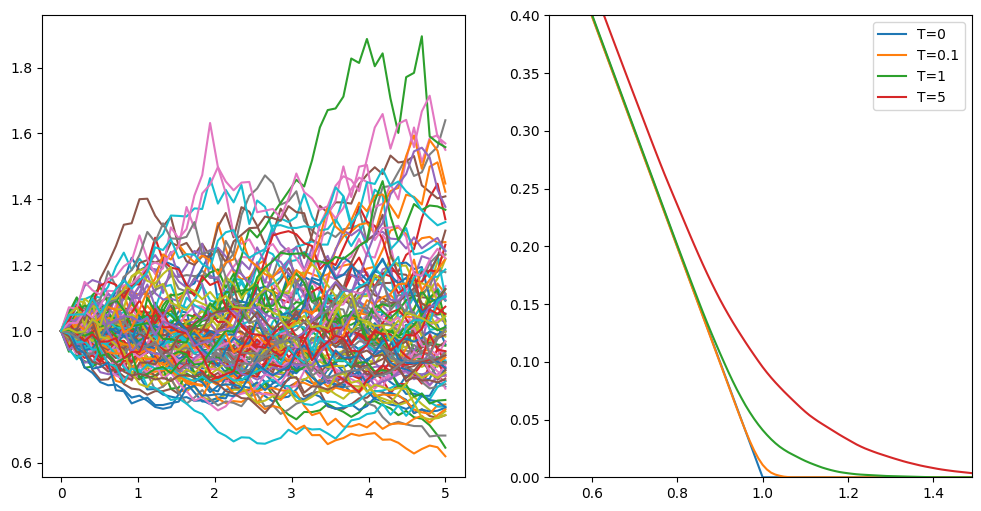
\includegraphics[width=0.8\linewidth]{addons/cev_sim}
\end{center}
\end{solution}

\end{questions}
\end{document}
